\section{Method}

\subsection{The singularity image}
A Singularity image needs a so called "receipt", which is a file that tells Singularity how to create the image and what to include in it. The recipe was added to Singularity Hub, an online library were Singularity receipts can be uploaded, which are then automatically built, so they can shared with other users \cite{singularity-hub}.

To complete the workflow from raw data to protein quantification results, several other software had to be included in the container, which are listed below.

\subsection{Quandenser} \label{ssec:quandenser-method}
 The core component in Quandenser-pipeline is Quandenser, which is a newly created software made in SciLifeLab by Lukas Käll and Matthew The, which condenses quantification data from label-free MS experiments by clustering both data from MS1 and MS2 without assigning identities to the values, thus decouples identification from quantification \cite{quandenser}. Due to Quandenser-pipeline can be run on clusters where singularity is installed (which is the case for UPPMAX), it opens up the possibility for parallelization which can in most cases significantly speed up the processing time.

A modified version of Quandenser was added to the pipeline, which can utilize parallel computation in conjunction with Nextflow's ability to run multiple processes in parallel. The improvements were integrated into the internal pipeline of Quandenser, which is shown in figure \ref{fig:quandenser-internal-pipeline}.

\begin{figure}[H]
  \centering
  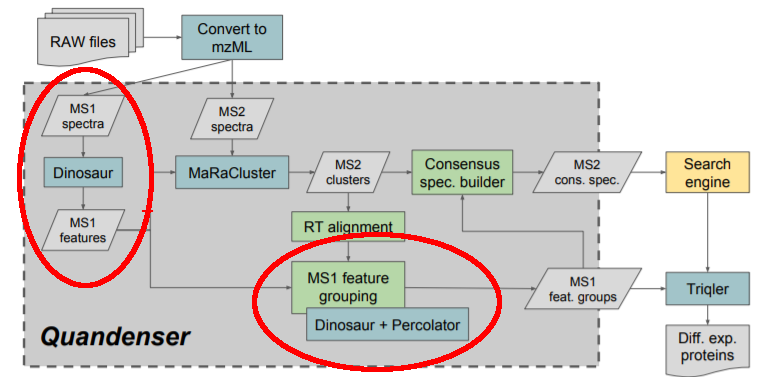
\includegraphics[width=\linewidth]{pictures/quandenser-internal.png}
  \caption{The internal pipeline of Quandenser (image from the Quandenser paper \cite{quandenser})}
  \label{fig:quandenser-internal-pipeline}
\end{figure}

Two parts were able to be parallelized within Quandenser's internal program. The parallelization works by adding stop points in the code to allow Nextflow to run part of the pipeline in parallel, spawning a new process of Quandenser each time. The first parallelizable part was "MS1 feature detection" with the internal program \textit{Dinosaur}, shown in figure \ref{fig:quandenser-internal-pipeline}. This is the first step in Quandenser's internal pipeline and was able to be "fully" parallelized, meaning that every process can be processed in parallel. The second part which was able to be parallelized was "MS1 feature grouping", shown in figure \ref{fig:quandenser-internal-pipeline}. This part of Quandenser could only be partially parallelized, due to the input files are calculated in a minimum spanning tree, a way to minimize the amount of connections and weights in a tree \cite{min-span-tree}. The reason behind why this is the case is that connecting branches cannot be calculated at the same time, while branches that are not directly connected can be processed in parallel. To cluster and process all files, the files must be calculated in a particular order according to the tree, while the Nextflow pipeline utilizes the minimum spanning tree output from Quandenser to create a processing tree that maximizes the amount of files that can be processed in parallel, given the order of the processes of Quandenser.

\subsubsection{MSconvert}
There exist a multitude of different types of MS data format, which can cause compatibility issues with existing software. The MS format depends on which instrument was used to generate the data, but most software cannot directly use any vendor-specific formatted files, meaning they have to be converted to a general MS data format first, most commonly files of type mzML \cite{mzml-format}. To combat the problem with incompatible data, a software named \textit{MSconvert} was added to the workflow, which can convert MS data from a multitude of vendor formats to the general MS data format needed to run Quandenser \cite{proteowizard}. Due to conversion from vendor formats with Msconvert only works on Windows operative systems, another solution was needed, since the Singularity image was based on Ubuntu, a Linux operative system. The solution was to use another type of software called \textit{Wine}, which adds an compatibility layer in Portable Operating System Interface (POSIX) systems, to run Windows software \cite{wine}. The Singularity image was based on another image created by the proteowizard developers, which incorporates all the necessary components to run Wine and MSconvert \cite{docker-image} \cite{docker-howto}.

\subsubsection{Crux}
Crux is an open source mass spectrometry analysis toolkit available for Linux, Windows and MacOS \cite{crux}. The purpose of integrating Crux into the image was to use three specific tools; tide-index, tide-search and percolator. Tide-index is a pre-search tool that adds indexes and decoys to the protein data base, which is used by the search tool tide-search, that parses fragmentation spectra and creates peptide-to-spectrum matches (PSMs) \cite{tide-search}. Percolator is a post-search tool, that separates peptide targets from decoy PSMs \cite{percolator}. In combination, the tools were used to post-process the output from Quandenser to prepare it for the software Triqler, explained in the next section.

\subsubsection{Triqler}
Triqler is an software which uses using graphical models and bayesian statistics to find differentially expressed proteins between samples. The main benefit with using Triqler in combination with Quandenser is that it utilizes both MS2 and MS1 spectra from the files, which improves the overall quantification of proteins \cite{triqler}.

% Add more here

\subsection{Nextflow}
Nextflow has integrated compatibility with running software inside Singularity images, meaning Nextflow can call on the programs contained within the Singularity image. The pipeline of Quandenser-pipeline is shown in figure \ref{fig:workflow}. As explained in section \ref{ssec:quandenser-method}, Nextflow's capability of running multiple processes in parallel was use with a modified version of Quandenser to allow for paralellization. When running the parallelized version of Quandenser in the pipeline, the processes are divided into five parts, two of which are parallelizable. The aim was to speed up the calculation time when running large cohorts, since the time scaling of an increased number of files was not a linear relationship to the processing time.

Nextflow also has the benefit of being able to submit processes to workload managers, which are used on HPC clusters to allocate processing time for users. To be able to run the pipeline on HPC clusters, the pipeline is outfitted with an option to enable submitting processes via SLURM, the current workload manager on UPPMAX.

\begin{figure}[H]
  \centering
  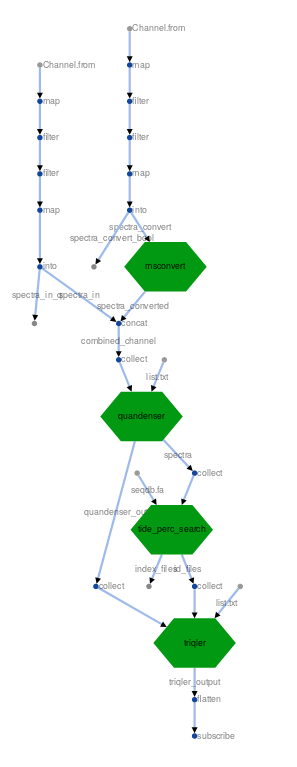
\includegraphics[width=0.5\linewidth]{pictures/workflow.png}
  \caption{Workflow of the pipeline. \textit{Batch file} is a file containing the paths to the mzML files and labels of the files to signify which are replicates}
  \label{fig:workflow}
\end{figure}

\subsection{Quandenser-pipeline Graphical User Interface (GUI)}
To integrate the Singularity image and the Nextflow pipeline, a GUI was created and packed into the image to improve the usability of the workflow, to allow users to easily modify and run the pipeline to their choosing. Pyside2 was used to create the GUI, which is an open source GUI framework based by the Qt framework \cite{pyside2}. Figure \ref{fig:GUI} illustrates how the GUI looks like and shows how different types of files (vendor specific files and mzML), can be used in the same pipeline without any need to convert the files beforehand.

\begin{figure}[H]
  \begin{center}
  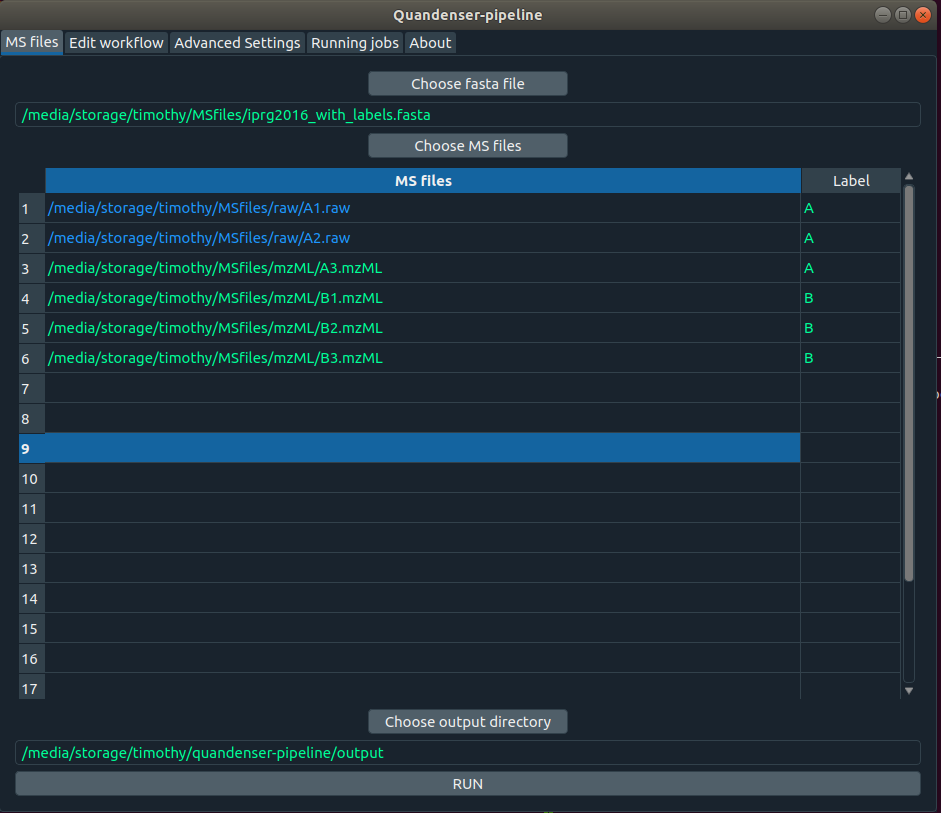
\includegraphics[height=10cm]{pictures/gui.png}
  \caption{GUI of Quandenser-pipeline}
  \label{fig:GUI}
  \end{center}
\end{figure}

To launch the GUI, a shell script handling installing Singularity, downloading the image from Singularity Hub and starting the GUI embedded inside the image. Figure \ref{fig:GUI_workflow} shows the GUI workflow. The GUI is used to modify the configurations for the pipeline, which affects how the pipeline is executed. When the user starts the pipeline, the GUI communicates to the shell script with a "named pipe", i.e a file which both the GUI and the shell script has access to, which tells the shell script to execute the Nextflow pipeline. The pipeline then calls on the Singularity image and executes the embedded software in the image at a particular order.

\begin{figure}[H]
  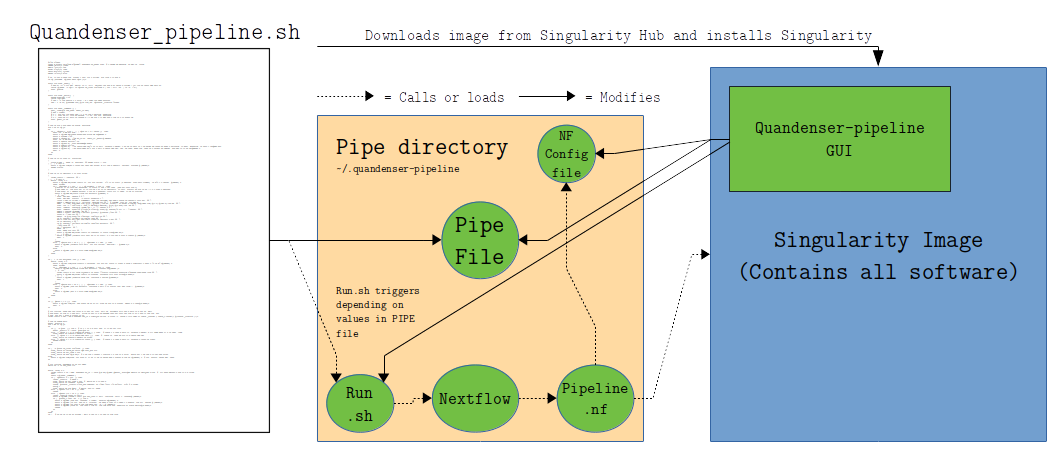
\includegraphics[width=\linewidth]{pictures/GUI_workflow.png}
  \caption{GUI workflow of Quandenser-pipeline}
  \label{fig:GUI_workflow}
\end{figure}

\subsection{Pipelines}
Two other pipelines using non-container software were tested on the bacterial proteome data. The following table illustrates which pipelines were used:

\newcommand{\textone}{\small The pipeline created for the thesis, using Quandenser as it's cornerstone. Due to Singularity not supporting non-POSIX systems, the Windows OS cannot run the pipeline natively without using a compatibility layer. An virtual machine wrapper was developed to allow users to run the pipeline in Windows}
\newcommand{\texttwo}{\small The custom pipeline tested on the data set was created by the workflow manager \textit{KNIME} in combination with \textit{OpenMS}, creating a custom workflow for analyzing mzML data \cite{knime} \cite{openms}. The pipeline was created by Michael Jahn at Paul Hudson's lab in SciLifeLab and was used to analyze bacterial data \cite{m-jahn-pipeline}. Both KNIME and OpenMS is available for Linux, MacOS and Windows.}
\newcommand{\textthree}{\small MaxQuant is a tool used for quantitative proteomics and is well suited for analyzing label-free proteomic data. The program can be run natively on Windows and on Linux with the framework \textit{Mono} \cite{maxquant} \cite{maxquant-installation}.}

\begin{table}[H]
\caption{Different pipelines used to compare Quandenser-pipeline}
\begin{center}
\begin{tabular}{|p{4cm}|p{9cm}|}
\hline
Program & Description \\ \hline \hline
Quandenser-pipeline v0.071 & \textone \\ \hline
KNIME + OpenMS & \texttwo \\ \hline
MaxQuant 1.6.3.3 & \textthree \\ \hline
\end{tabular}
\end{center}
\end{table}

\subsection{Analyzing bacterial proteomes}
The two data sets were generated in Paul Hudson's lab at SciLifeLab. The first data set were generated by letting cyanobacteria grow in five different simulated environments (before dawn, after dawn, noon, before sunset and after sunset) with two replicates each. The second bacterial data set was ralstonia bacteria being grown in a chemostat bioreactor where Formic Acid (FA) was limited during the experiment, in five different conditions (0.05, 0.10, 0.15, 0.20 and 0.25 growth-rate) with four replicates each.

The RAW data files for the cyanobacteria data set and ralstonia data set was on average 0.8 Gb respectively 1.3 Gb in size. Both data sets were run on different established proteomic pipelines to compare the performance of the newly created pipeline.

Significantly differentially expressed proteins were also analyzed from the cyanobacteria data set. To define a differentially expressed protein, a relevant statistical parameter was chosen to represent how statistically significant find is; the q-value. A q-value is an excellent statistical measurement when doing multiple tests, which in this case is for each specific protein \cite{q-value}. The threshold of a differentially expressed protein was set as a q-value less than 0.05. In contrary to the p-value, a p-value threshold of 0.05 means 5\% of all tests will result in a false positives while a q-value threshold of 0.05 will result in 5\% of all \textit{significant} differentially expressed results being false positives \cite{q-value}. Triqler, which was included in the pipeline, will automatically calculate q-values of proteins, and a threshold of a q-value of 0.05 was set as "differentially expressed".
